% Section content template for individual Educative lessons
% This file contains the actual content for a specific section
% Generated from Educative API section content

% Section: Design of a Distributed Logging Service
% Section ID: 4835612456124416
% Section Slug: design-of-a-distributed-logging-service
% Generated: 2025-12-07T22:01:42.509340

We'll design the distributed logging system now. Our logging system should log all activities or messages (we'll not incorporate sampling ability into our design).

\subsection{Requirements}\label{kTa1KW306-JF2wjlKZIU8}
\\
Let's list the requirements for designing a distributed logging system:

\subsubsection{Functional requirements}\label{NAVvSH5Pk1Z2ZfV-Wnhwl}
\\
The functional requirements of our system are as follows:

\begin{itemize}
\item
\protect\phantomsection\label{W4Jpg2Q9CTLEGRZ_XqOoI}
\textbf{Writing logs}: The services of the distributed system must be able to write into the logging system.
\item
\protect\phantomsection\label{-bwcr33oCMvbeW5PDoM3T}
\textbf{Searchable logs}: It should be effortless for a system to find logs. Similarly, the application's flow from end-to-end should also be effortless.
\item
\protect\phantomsection\label{GYYXwiN1ENOm2lpTigPd7}
\textbf{Storing logging}: The logs should reside in distributed storage for easy access.
\item
\protect\phantomsection\label{1_qRswxoNFYOmhcLm3W22}
\textbf{Centralized logging visualizer}: The system should provide a unified view of globally separated services.
\end{itemize}

\subsubsection{Non-functional requirements}\label{3nkbDFBrrPar9rUQMiEV-}
\\
The non-functional requirements of our system are as follows:

\begin{itemize}
\item
\protect\phantomsection\label{O1MIQRnrxJX9TTArB81mU}
\textbf{Low latency}: Logging is an I/O-intensive operation that is often much slower than CPU operations. We need to design the system so that logging is not on an application's critical path.
\item
\protect\phantomsection\label{dkRONGDcIChMt2_Mn_a74}
\textbf{Scalability:} We want our logging system to be scalable. It should be able to handle the increasing amounts of logs over time and a growing number of concurrent users.
\item
\protect\phantomsection\label{NCw5jBc6ZFi55lViixTtf}
\textbf{Availability:} The logging system should be highly available to log the data.
\end{itemize}

\subsection{Building blocks we will use}\label{zjuybuoBQ2m11_kd2T_hq}
\\
The design of a distributed logging system will utilize the following building blocks:

\begin{itemize}
\item
\protect\phantomsection\label{sEjD9spp4DrF8mybMthtF}
\href{https://www.educative.io/courses/grokking-the-system-design-interview/system-design-the-pub-sub-abstraction}{\textbf{Pub-sub system}}: We'll use a pub-sub- system to handle the huge size of logs.
\item
\protect\phantomsection\label{4d2ZSn2vmYfuhB-3nCAo6}
\href{https://www.educative.io/courses/grokking-the-system-design-interview/system-design-the-distributed-search}{\textbf{Distributed search}}: We'll use distributed search to query the logs efficiently.
\end{itemize}

\begin{figure}[htbp]
 \centering
 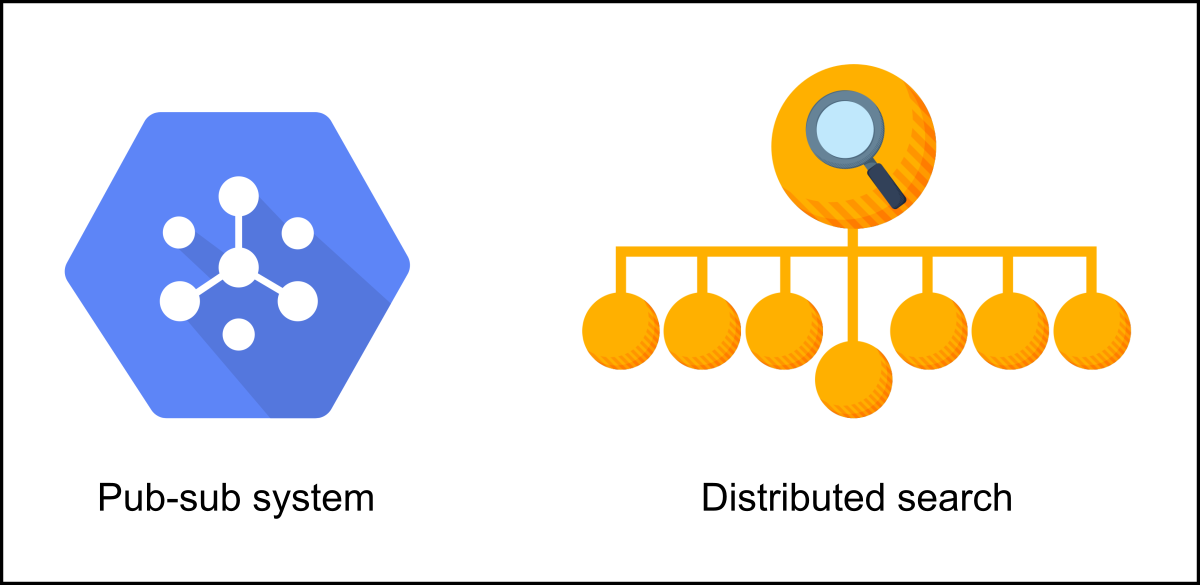
\includegraphics[width=0.15\textwidth]{Images/chapter_22/section_4835612456124416/6713440498745344.png}
 \caption{Building blocks we will use}
\end{figure}

\subsection{API design}\label{T6SN34_jWkwPxn43Xtoar}
\\
The API design for this problem is given below:

\subsubsection{Write a message}\label{nUnCV8w31Tn7THCqYZd2a}
\\
The API call to perform writing should look like this:

\begin{lstlisting}[language=JavaScript]
write(unique_ID, message_to_be_logged)
\end{lstlisting}

\begin{table}[htbp]
\centering
\small
\adjustbox{max width=\textwidth}{
\begin{tabular}{|p{0.253\textwidth}|p{0.697\textwidth}|}
\hline
\textbf{Parameter} & \textbf{Description} \\
\hline
\hline
\texttt{unique\_ID} & It is a numeric ID containing \texttt{application-id}, \texttt{service-id,} and a time stamp. \\
\hline
\texttt{message\_to\_be\_logged} & It is the log message stored against a unique key. \\
\hline
\end{tabular}
}
\end{table}

\subsubsection{Search log}\label{XoEvOd5QhIk-4zLmVA7FF}
\\
The API call to search data should look like this:

\begin{lstlisting}[language=JavaScript]
searching(keyword)
\end{lstlisting}

This call returns a list of logs that contain the keyword.

\begin{table}[htbp]
\centering
\small
\adjustbox{max width=\textwidth}{
\begin{tabular}{|p{0.256\textwidth}|p{0.694\textwidth}|}
\hline
\textbf{Parameter} & \textbf{Description} \\
\hline
\hline
\texttt{keyword} & It is used for finding the logs containing the \texttt{keyword}. \\
\hline
\end{tabular}
}
\end{table}

\subsection{Initial design}\label{RkA-cf_cPf_y_KwzHfAYi}
\\
In a distributed system, clients across the globe generate events by requesting services from different serving nodes. The nodes generate logs while handling each of the requests. These logs are accumulated on the respective nodes.
\\
In addition to the building blocks, let's list the major components of our system:

\begin{itemize}
\item
\protect\phantomsection\label{2n4yvJ9Pv2DSx4FEFYxFP}
\textbf{Log accumulator}: An agent that collects logs from each node and dumps them into storage. So, if we want to know about a particular event, we don't need to visit each node, and we can fetch them from our storage.
\item
\protect\phantomsection\label{p6JJM38TppLsYE8QLkTX7}
\textbf{Storage}: The logs need to be stored somewhere after accumulation. We'll choose blob storage to save our logs.
\item
\protect\phantomsection\label{eK_RyRJN2ge_clqQghmcg}
\textbf{Log indexer}: The growing number of log files affects the searching ability. The log indexer will use the distributed search to search efficiently.
\item
\protect\phantomsection\label{A8flTvtB7kl117n447909}
\textbf{Visualizer}: The visualizer is used to provide a unified view of all the logs.
\end{itemize}
\\
The design for this method looks like this:

\begin{figure}[htbp]
 \centering
 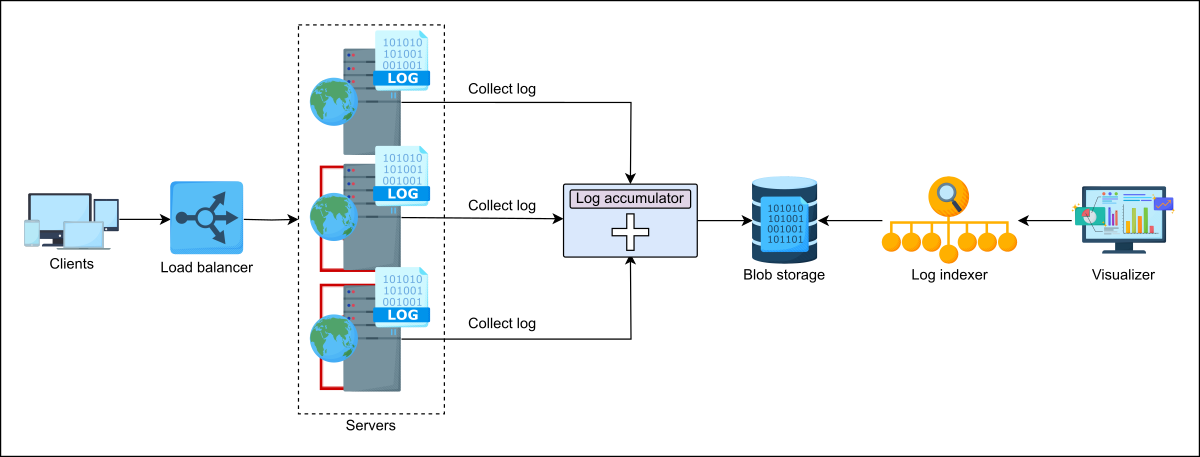
\includegraphics[width=0.5\textwidth]{Images/chapter_22/section_4835612456124416/6533710847803392.png}
 \caption{High-level design}
\end{figure}

There are millions of servers in a distributed system, and using a single log accumulator severely affects scalability. Let 's learn how we'll scale our system.

\subsection{Logging at various levels}\label{mVul9oJ3V28jPyMCk46uj}
\\
Let's explore how the logging system works at various levels.

\subsubsection{In a server}\label{pJUaCJVQVzoPzBEDyifsb}
\\
In this section, we'll learn how various services belonging to different apps will log in to a server.
\\
Let's consider a situation where we have multiple different applications on a server, such as App 1, App 2, and so on. Each application has various microservices running as well. For example, an e-commerce application can have services like authenticating users, fetching carts, and more running at the same time. Every service produces logs. We use an ID with \texttt{application-id}, \texttt{service-id}, and its time stamp to uniquely identify various services of multiple applications. Time stamps can help us to determine the causality of events.
\\
Each service will push its data to the \textbf{log accumulator} service. It is responsible for these actions:

\begin{itemize}
\item
\protect\phantomsection\label{Dkn7rxM9u8Ve-U1qnxo9n}
Receiving the logs.
\item
\protect\phantomsection\label{kdfB_rlv7eXijl0b7pbN6}
Storing the logs locally.
\item
\protect\phantomsection\label{GOsY6JG-3WyH95BPBCHb4}
Pushing the logs to a \href{https://www.educative.io/courses/grokking-the-system-design-interview/system-design-the-pub-sub-abstraction}{pub-sub system}.
\end{itemize}
\\
We use the pub-sub system to cater to our scalability issue. Now , each server has its log accumulator (or multiple accumulators) push the data to pub-sub. The pub-sub system is capable of managing a huge amount of logs.
\\
To fulfill another requirement of low latency, we don't want the logging to affect the performance of other processes, so we send the logs asynchronously via a low-priority thread. By doing this, our system does not interfere with the performance of others and ensures availability.

\begin{figure}[htbp]
 \centering
 \begin{subfigure}[b]{0.48\textwidth}
 \centering
 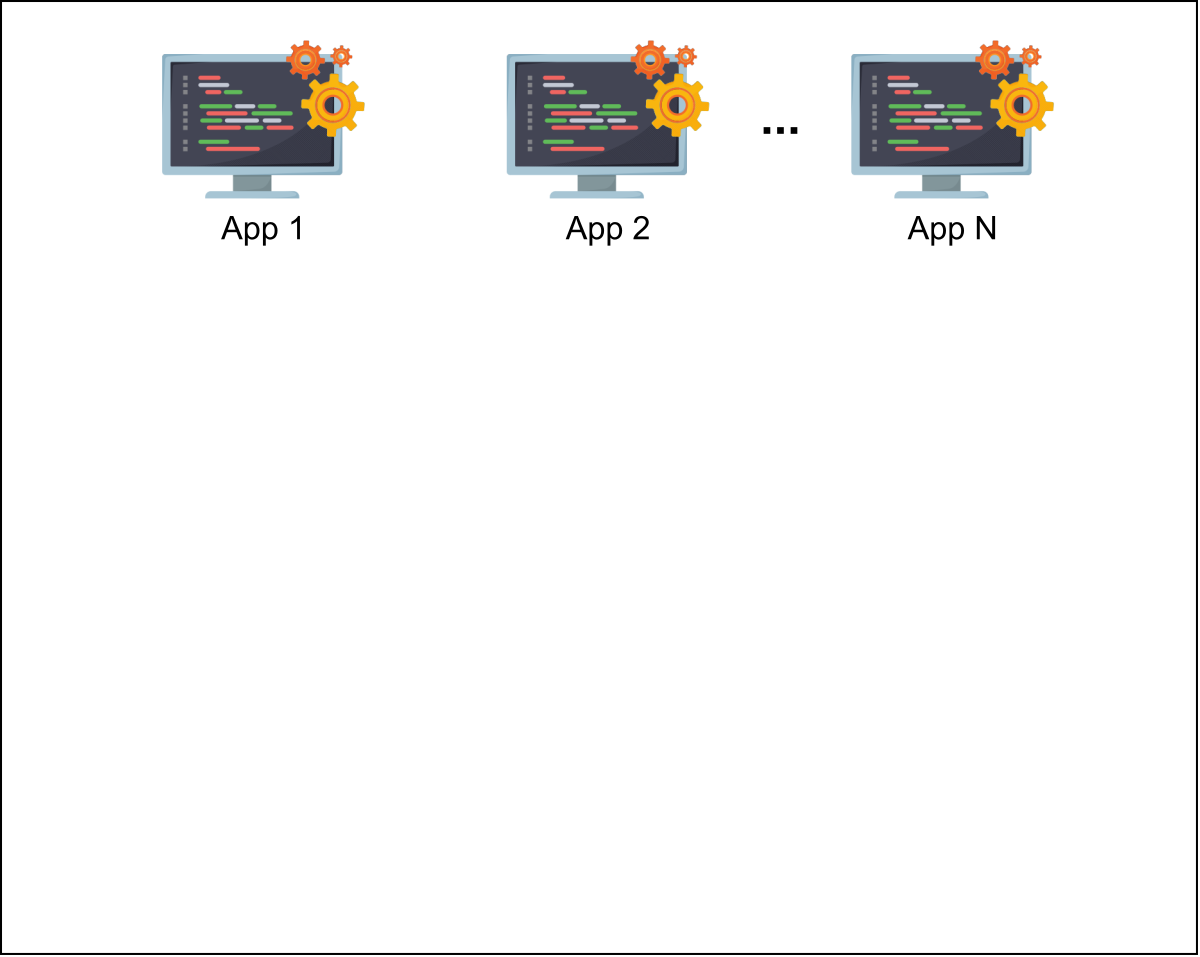
\includegraphics[width=\textwidth]{Images/chapter_22/section_4835612456124416/6504623852879872.png}
 \caption{Multiple applications running on a server, and each application has various microservices.}
 \end{subfigure}
 \hfill
 \begin{subfigure}[b]{0.48\textwidth}
 \centering
 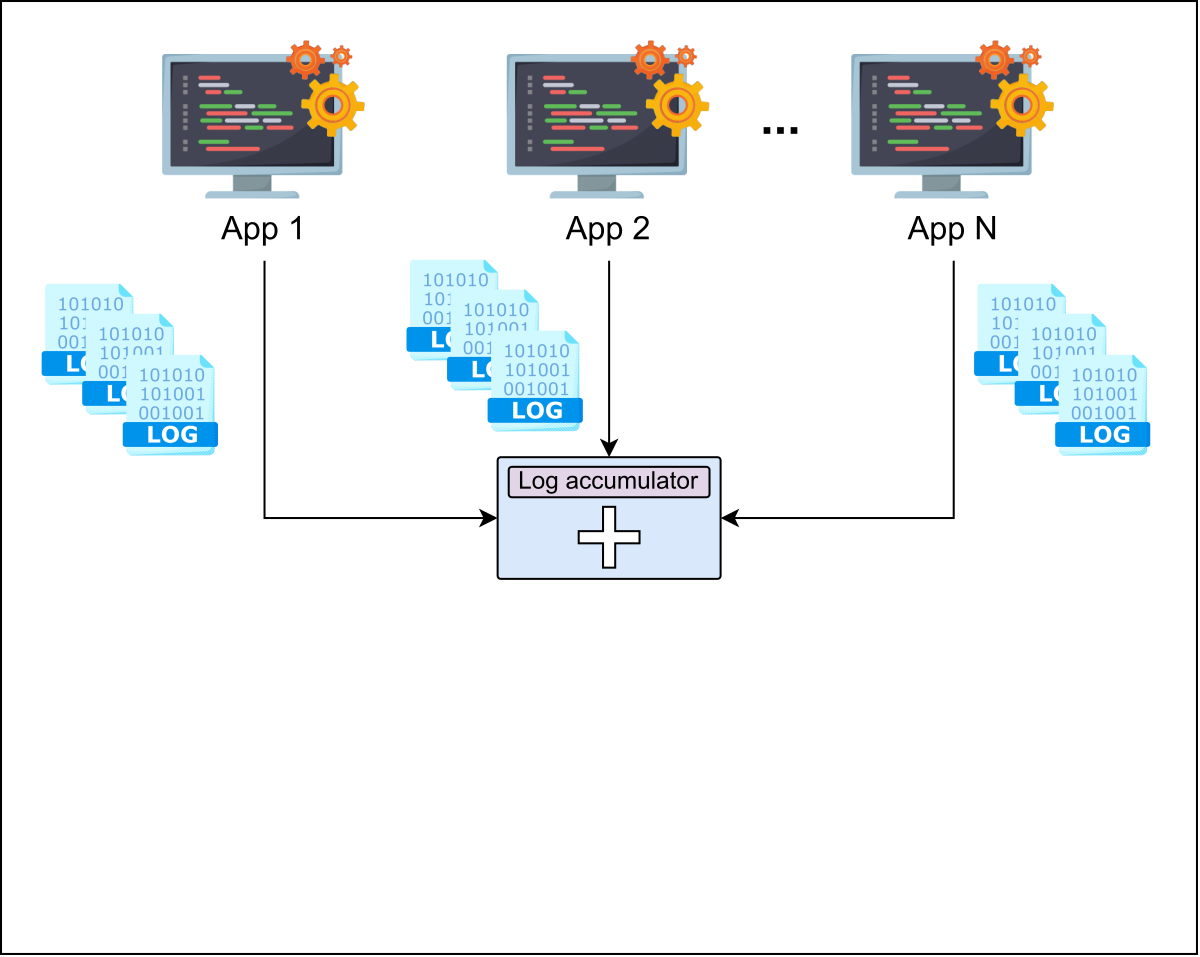
\includegraphics[width=\textwidth]{Images/chapter_22/section_4835612456124416/5757862855180288.png}
 \caption{Each service produces logs and sends them to the log accumulator}
 \end{subfigure}
\end{figure}

\begin{figure}[htbp]
 \centering
 \begin{subfigure}[b]{0.48\textwidth}
 \centering
 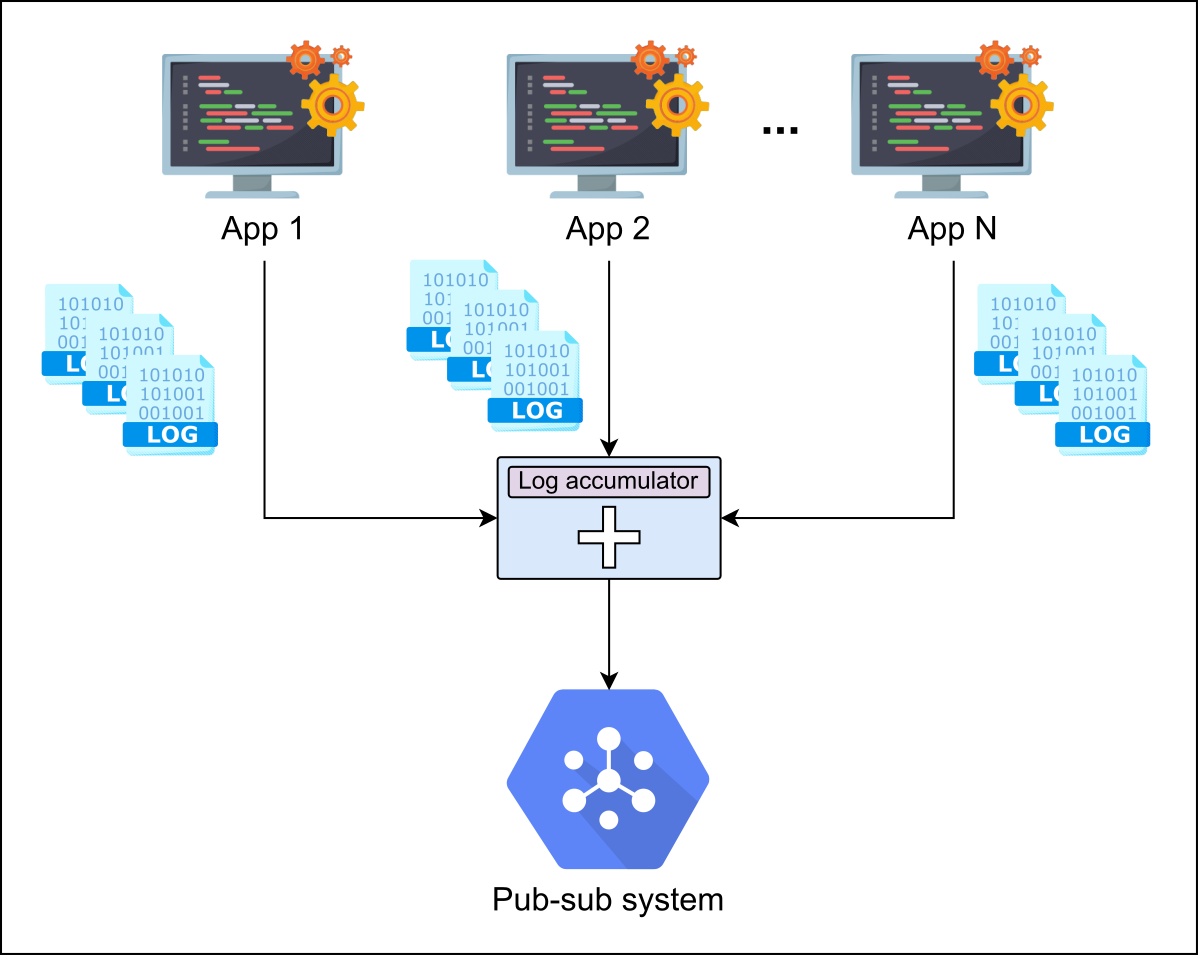
\includegraphics[width=\textwidth]{Images/chapter_22/section_4835612456124416/4993183019040768.png}
 \caption{Log accumulator pushes logs to a pub-sub system.}
 \end{subfigure}
\end{figure}

We should be mindful that data can be lost in the process of logging huge amounts of messages. There is a trade-off between user-perceived latency and the guarantee that log data persists. For lower latency, log services often keep data in RAM and persist them asynchronously. Additionally , we can minimize data loss by adding redundant log accumulators to handle growing concurrent users.\\

\begin{quote}
\textbf{Quiz:}
\textbf{Question 1:} How does logging change when we host our service on a multi-tenant cloud

(like AWS) versus when an organization has exclusive control of the infrastructure (like Facebook), specifically in terms of logs?
\textbf{Answer:} Security might be one aspect that differs between multi-tenant and single-tenant settings. When we encrypt all logs and secure a logging service end-to-end, it does not come free, and has performance penalties. Additionally, strict separation of logs is required for a multi-tenant setting, while we can improve the storage and processing utilization for a single-tenant setting. Let's take the example of

Meta's Facebook. They have millions of machines that generate logs, and the size of the logs can be several petabytes per hour. So, each machine pushes its logs to a pub-sub system named Scribe. Scribe retains data for a few days and various other systems process the information residing in the Scribe. They store the logs in distributed storage also. Managing the logs can be application-specific. On the other hand, for multi-tenancy, we need a separate instance of pub-sub per tenant (or per application) for strict separation of logs.
\end{quote}

\begin{quote}
\textbf{Note:} For applications like banking and financial apps, the logs must be very secure so hackers cannot steal the data. The common practice is to encrypt the data and log. In this way, no one can decrypt the encrypted information using the data from logs.
\end{quote}
\subsubsection{At datacenter level}\label{wIe0GMqi9juhv8TGA5GlI}
\\
All servers in a data center push the logs to a pub-sub system. Since we use a horizontally-scalable pub-sub system, it is possible to manage huge amounts of logs. We may use multiple instances of the pub-sub per data center. It makes our system scalable, and we can avoid bottlenecks. Then , the pub-sub system pushes the data to the blob storage.\\

\begin{figure}[htbp]
 \centering
 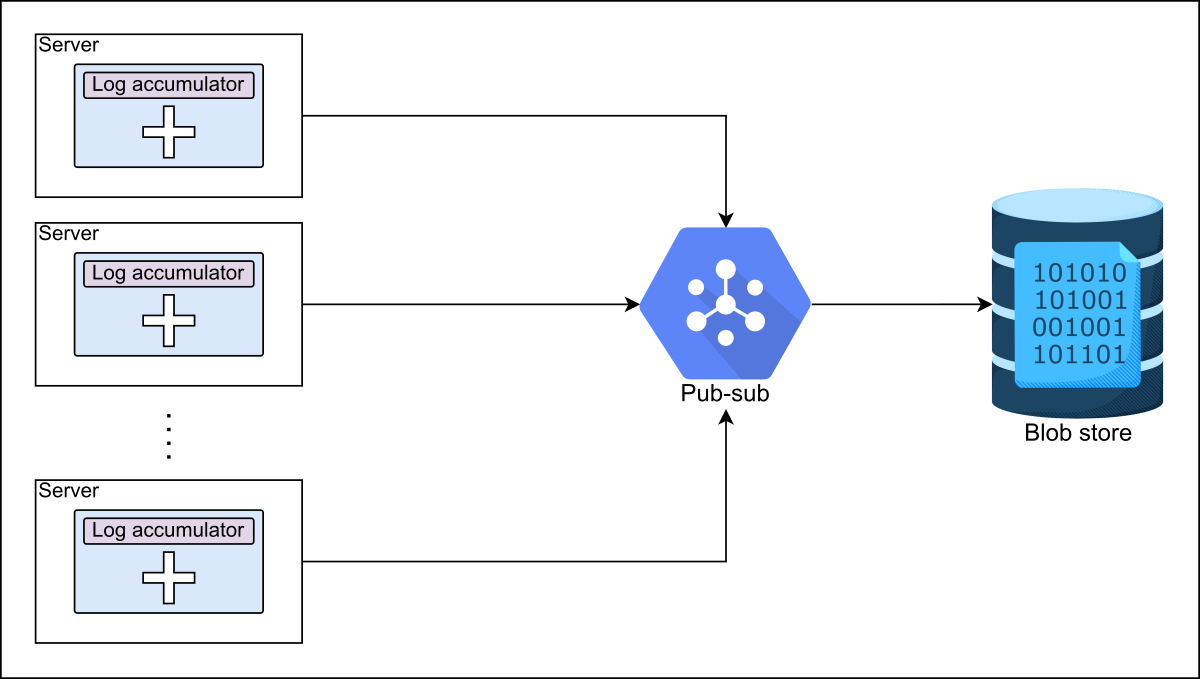
\includegraphics[width=0.5\textwidth]{Images/chapter_22/section_4835612456124416/6018768092659712.png}
 \caption{Log accumulator sending data to the pub-sub system}
\end{figure}

The data does not reside in pub-sub forever and gets deleted after a few days before being stored in archival storage. However, we can utilize the data while it is available in the pub-sub system. The following services will work on the pub-sub data:

\begin{itemize}
\item
\protect\phantomsection\label{-KUk0MbQrNl2t1BnSYd8m}
\textbf{Filterer}: It identifies the application and stores the logs in the blob storage reserved for that application since we do not want to mix logs of two different applications.
\item
\protect\phantomsection\label{cZCXVh3w3D-bC_WTBWkOc}
\textbf{Error aggregator}: It is critical to identify an error as quickly as possible. We use a service that picks up the error messages from the pub-sub system and informs the respective client. It saves us the trouble of searching the logs.
\item
\protect\phantomsection\label{yVpi5D2nSx7-2_K5P07VT}
\textbf{Alert aggregator}: Alerts are also crucial. So, it is important to be aware of them early. This service identifies the alerts and notifies the appropriate stakeholders if a fatal error is encountered, or sends a message to a monitoring tool.
\end{itemize}
\\
The updated design is given below:

\begin{figure}[htbp]
 \centering
 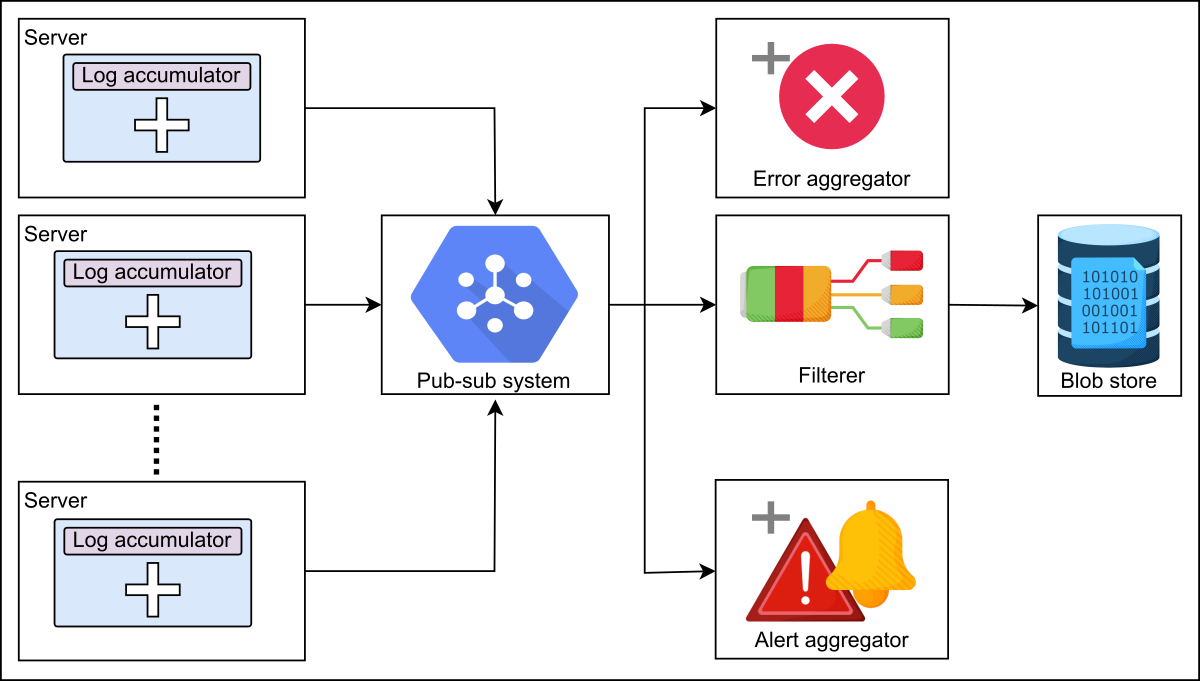
\includegraphics[width=0.5\textwidth]{Images/chapter_22/section_4835612456124416/5879527853391872.png}
 \caption{Adding a filterer, error aggregator, and alert aggregator}
\end{figure}

\begin{quote}
\textbf{Quiz:}
\textbf{Question 1:} Do we store the logs for a lifetime?
\textbf{Answer:} Logs also have an expiration date. We can delete regular logs after a few days or months. Compliance logs are usually stored for up to three to five years. It depends on the requirements of the application.
\end{quote}

In our design, we have identified another component called the \textbf{expiration checker}. It is responsible for these tasks:

\begin{itemize}
\item
\protect\phantomsection\label{0TvPuVwIXnN5BsnUNnDW6}
Verifying the logs that have to be deleted. Verifying the logs to store in cold storage(Cold storages are low-cost storages where archived data is kept. It is done to save money on storage charges and to migrate data that isn't used frequently.).
\end{itemize}
\\
Moreover, our components log indexer and visualizer work on the blob storage to provide a good searching experience to the end user. We can see the final design of the logging service below:

\begin{figure}[htbp]
 \centering
 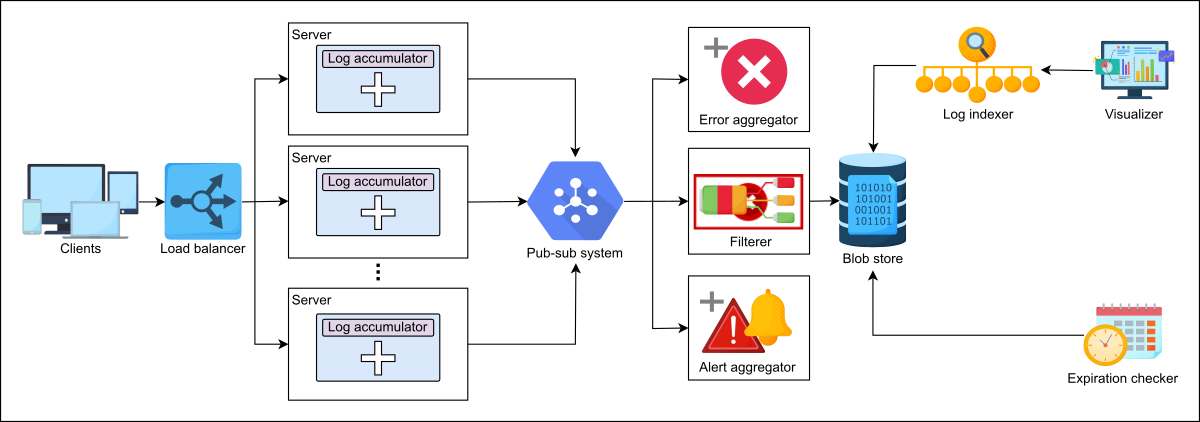
\includegraphics[width=0.5\textwidth]{Images/chapter_22/section_4835612456124416/5832048785096704.png}
 \caption{Logging service design}
\end{figure}

\begin{quote}
\textbf{Quiz:}
\textbf{Question 1:} We learned earlier that a simple user-level API call to a large service might involve hundreds of internal microservices and thousands of nodes.

How can we stitch together logs end-to-end for one request with causality intact?
\textbf{Answer:} Most complex services use a front-end server to handle an end user's request. On reception of a request, the front-end server can get a unique identifier using a sequencer. This unique identifier will be appended to all the fanned-out services. Each log message generated anywhere in the system also emits the unique identifier. Later, we can filter the log (or preprocess it) based on the unique identifiers. At this step, we are able to collect all the logs across microservices against a unique request. In the building block, we discussed that we can get unique identifiers that maintain happens-before causality. Such an identifier has the property that if ID 1 is less than ID 2, then ID 1 represents a time that occurred before ID 2. Now, each log item can use a time- stamp, and we can sort log entries for a specific request in ascending order.
Correctly ordering the log in a chronological (or causal) order simplifies log analyses.
\end{quote}

\begin{quote}
\textbf{Note:} Windows Azure Storage System (WAS) uses an extensive logging infrastructure in its development. It stores the logs in local disks, and given a large number of logs, they do not push the logs to the distributed storage. Instead, they use a grep-like utility that works as a distributed search. This way, they have a unified view of globally distributed logs data.
\end{quote}
\\
There can be various ways to design a distributed logging service, but it solely depends on the requirements of our application.
\\
How would you design a distributed logging system for a high-traffic online banking application, ensuring security, performance, and scalability are optimized for critical operations?\\

\subsection{Conclusion}\label{m-tNY4snR8QznMZJ-wQ6c}

\begin{itemize}
\item
\protect\phantomsection\label{kQRFk5wZAkN9v3_L9GB-0}
We learned how logging is crucial in understanding the flow of events in a distributed system. It helps to reduce the mean time to repair (MTTR) by steering us toward the root causes of issues.
\item
\protect\phantomsection\label{dFgjMj0M_tVVC0cl8XEVc}
Logging is an I/O-intensive operation that is time-consuming and slow. It is essential to handle it carefully and not affect the critical path of other services' execution.
\item
\protect\phantomsection\label{d-UUuM_ruuGZC7YkeyxSG}
Logging is essential for monitoring because the data fetched from logs helps monitor the health of an application. (Alert and error aggregators serve this purpose.)
\end{itemize}

% End of section content